\usetikzlibrary{arrows.meta,decorations.markings,patterns}

\providecommand{\computer}{%
    
\includegraphics[width=1cm]{../common/Noun_project_216.pdf}
}
\providecommand{\switch}{%
    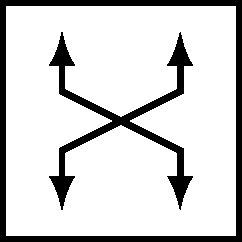
\includegraphics[width=0.9cm]{../common/fig-switch.pdf}
}
\providecommand{\router}{%
    
\includegraphics[width=0.9cm]{../common/fig-router.pdf}
}

\begin{frame}
\frametitle{recall: broadcast}
\begin{itemize}
\item MAC address FF:FF:FF:FF:FF:FF = everyone on network
\item `simple' implementation: send to all but incoming port
\vspace{.5cm}
\item one way to do this in P4:
    \begin{itemize}
    \item setup multicast group that includes all ports
    \item send to that multicast group in ingress processing
    \item drop the packet in egress processing if port number matches incoming port
    \end{itemize}
\end{itemize}
\end{frame}

\begin{frame}[label=noBackwardsQ]{aside: no backwards broadcast}
    \begin{itemize}
    \item broadcast \textit{sent to all but incoming port}
    \item question: what would happen if we didn't do this?
        \begin{itemize}
        \item multiple may apply
        \end{itemize}
    \end{itemize}
\begin{tabular}{l}
A. might cause host to receive duplicates \\
B. might cause copies sent to non-incoming port to be dropped \\
C. might cause frames sent at same time to be dropped \\
D. might cause frames sent much later to be dropped \\
\end{tabular}
\end{frame}

\begin{frame}[fragile]{loop from backwards broadcast}
\begin{tikzpicture}[remember picture]
\tikzset{
    computer/.style={inner sep=0mm,outer sep=0mm,execute at begin node={\computer}},
    switch/.style={inner sep=0mm,outer sep=0mm,execute at begin node={\switch}},
    connect/.style={draw,very thick,Latex-Latex},
    connect big/.style={draw,ultra thick,Latex-Latex},
    port/.style={pos=0.95,fill=white,circle,draw,inner sep=0mm},
    port beginning/.style={pos=0.05,fill=white,circle,draw,inner sep=0mm},
    mac label/.style={
        draw,fill=white,inner sep=1mm,font=\tiny\tt,
    },
    one packet/.style n args={3}{
        alt={<#1>{
            postaction=decorate,
            decoration={
                markings,
                mark={at position .5 with
                    \node[
                        thin,transform shape,draw,
                        preaction={fill=white},
                        pattern=crosshatch,pattern color=blue!50,font=\tt,#2
                    ]{#3};
                }
            }
        }},
    },
    one packet forward/.style 2 args={
        one packet={#1}{#2}{>>>},
    },
    one packet backward/.style 2 args={
        one packet={#1}{#2}{<<<},
    },
    hilite/.style={
        alt=<#1>{preaction={fill=red!20},pattern=none},
    },
}
\node[overlay,anchor=north east] at ([xshift=-1cm]current page.north east) {
    time step \myemph{\large\insertoverlaynumber}
};
\foreach \x/\d/\mc/\dir in {15/8cm/AA/north,45/3cm/BB/north,90/2cm/CC/north,135/3cm/DD/north,180/4cm/EE/north,300/4cm/FF/south} {
    \node[computer,label={[mac label,]\dir:00:11:22:33:44:\small\mc},alias=c-\mc] (c-\x) at (\x:\d) {};
}
\node[switch] (s1) at (4,-0.5) {};
\node[switch] (s2) at (-1,-2.5) {};
\draw[connect,one packet forward=1,one packet backward={2}{hilite=2}] (c-15) -- (s1) node[port] {1};
\draw[connect,one packet backward=2,one packet backward=4] (c-45) -- (s1) node[port] {2};
\draw[connect,one packet backward=2,one packet backward=4] (c-300) -- (s1) node[port] {3};
\draw[connect,one packet backward=3] (c-90) -- (s2) node[port] {2};
\draw[connect,one packet backward=3] (c-135) -- (s2) node[port] {3};
\draw[connect,one packet backward=3] (c-180) -- (s2) node[port] {4};
\draw[connect big,one packet forward=2,one packet backward={3}{hilite=3},one packet forward={4}{hilite=4}] (s1) -- (s2) node[port beginning] {4} node [port] {1};
\end{tikzpicture}
\end{frame}

\begin{frame}{loops}
    \begin{itemize}
    \item each packet keeps getting sent indefinitely
    \item remember: happens for \textit{every packet sent}
    \item quickly overwhelms link between switches
    \vspace{.5cm}
    \item but can just avoid by not sending back?
    \end{itemize}
\end{frame}

\begin{frame}[fragile]{loops with only-to-other}
\begin{tikzpicture}[remember picture]
\tikzset{
    computer/.style={inner sep=0mm,outer sep=0mm,execute at begin node={\computer}},
    switch/.style={inner sep=0mm,outer sep=0mm,execute at begin node={\switch}},
    connect/.style={draw,very thick,Latex-Latex},
    connect big/.style={draw,ultra thick,Latex-Latex},
    port/.style={pos=0.95,fill=white,circle,draw,inner sep=0mm},
    port beginning/.style={pos=0.05,fill=white,circle,draw,inner sep=0mm},
    mac label/.style={
        draw,fill=white,inner sep=1mm,font=\tiny\tt,
    },
    one packet/.style n args={3}{
        alt={<#1>{
            postaction=decorate,
            decoration={
                markings,
                mark={at position .5 with
                    \node[
                        thin,transform shape,draw,
                        preaction={fill=white},
                        pattern=crosshatch,pattern color=blue!50,font=\tt,#2
                    ]{#3};
                }
            }
        }},
    },
    two packet/.style n args={3}{
        alt={<#1>{
            postaction=decorate,
            decoration={
                markings,
                mark={at position .3 with
                    \node[
                        thin,transform shape,draw,
                        preaction={fill=white},
                        pattern=crosshatch,pattern color=blue!50,font=\tt,#2
                    ]{#3};
                },
                mark={at position .6 with
                    \node[
                        thin,transform shape,draw,dashed,
                        preaction={fill=white},
                        pattern=crosshatch,pattern color=blue!50,font=\tt,#2
                    ]{#3};
                }
            }
        }},
    },
    one packet forward/.style 2 args={
        one packet={#1}{#2}{>>>},
    },
    one packet backward/.style 2 args={
        one packet={#1}{#2}{<<<},
    },
    one packet both/.style 2 args={
        one packet={#1}{#2}{<</>>},
    },
    hilite/.style={
        alt=<#1>{preaction={fill=red!20},pattern=none},
    },
    hilite b/.style={
        alt=<#1>{dashed,preaction={fill=red!20},pattern=none},
    },
    hilite alt/.style={
        alt=<#1>{pattern=north west lines,pattern color=black!50},
    },
}
\node[overlay,anchor=north east] at ([xshift=-1cm]current page.north east) {
    time step \myemph{\large\insertoverlaynumber}
};
\foreach \x/\d/\mc/\dir in {15/8cm/AA/north,30/4cm/BB/north,90/2cm/CC/north,135/3cm/DD/north,180/4cm/EE/north,46/2cm/FF/north} {
    \node[computer,label={[mac label,]\dir:00:11:22:33:44:\small\mc},alias=c-\mc] (c-\x) at (\x:\d) {};
}
\node[switch] (s1) at (2.5,-0.5) {};
\node[switch] (s2) at (-1,-0.5) {};
\node[switch] (s3) at (6,-3.5) {};
\draw[connect,one packet forward=1,two packet={5}{}{<<<}] (c-15) -- (s3);
\draw[connect,one packet backward=2,two packet={5}{}{<<<}] (c-BB) -- (s3);
\draw[connect,one packet backward=3,
      one packet backward={4}{hilite alt=4},
      ] (c-FF) -- (s1);
\draw[connect,one packet backward=3,
      one packet backward={4}{hilite alt=4},
      ] (c-90) -- (s2);
\draw[connect,one packet backward=3,
      one packet backward={4}{hilite alt=4},
     ] (c-135) -- (s2);
\draw[connect,one packet backward=3,
      one packet backward={4}{hilite alt=4},
      ] (c-180) -- (s2);
\draw[connect big,one packet both={3}{hilite=3},] (s1) -- (s2);
\draw[connect big,one packet backward=2,one packet forward={4}{hilite b=4},
    one packet backward={5}{hilite=5}] (s1) -- (s3);
\draw[connect big,one packet backward={2}{hilite=2},
    one packet forward={4}{hilite=4},
    one packet backward={5}{hilite b=5}] (s2) -- (s3);
\end{tikzpicture}
\end{frame}

\begin{frame}{explosion from loops}
\begin{itemize}
\item avoiding sending back is not enough
\item will get catastrophic failure of network!
\vspace{.5cm}
\item simple fix: only have one path from A to B
    \begin{itemize}
    \item BUT means network is more fragile
    \end{itemize}
\item we'll have better solutions when we talk about routing later
\end{itemize}
\end{frame}
